
\begin{figure*}[h]
    \centering
    \begin{minipage}{0.45\textwidth}
        \centering
        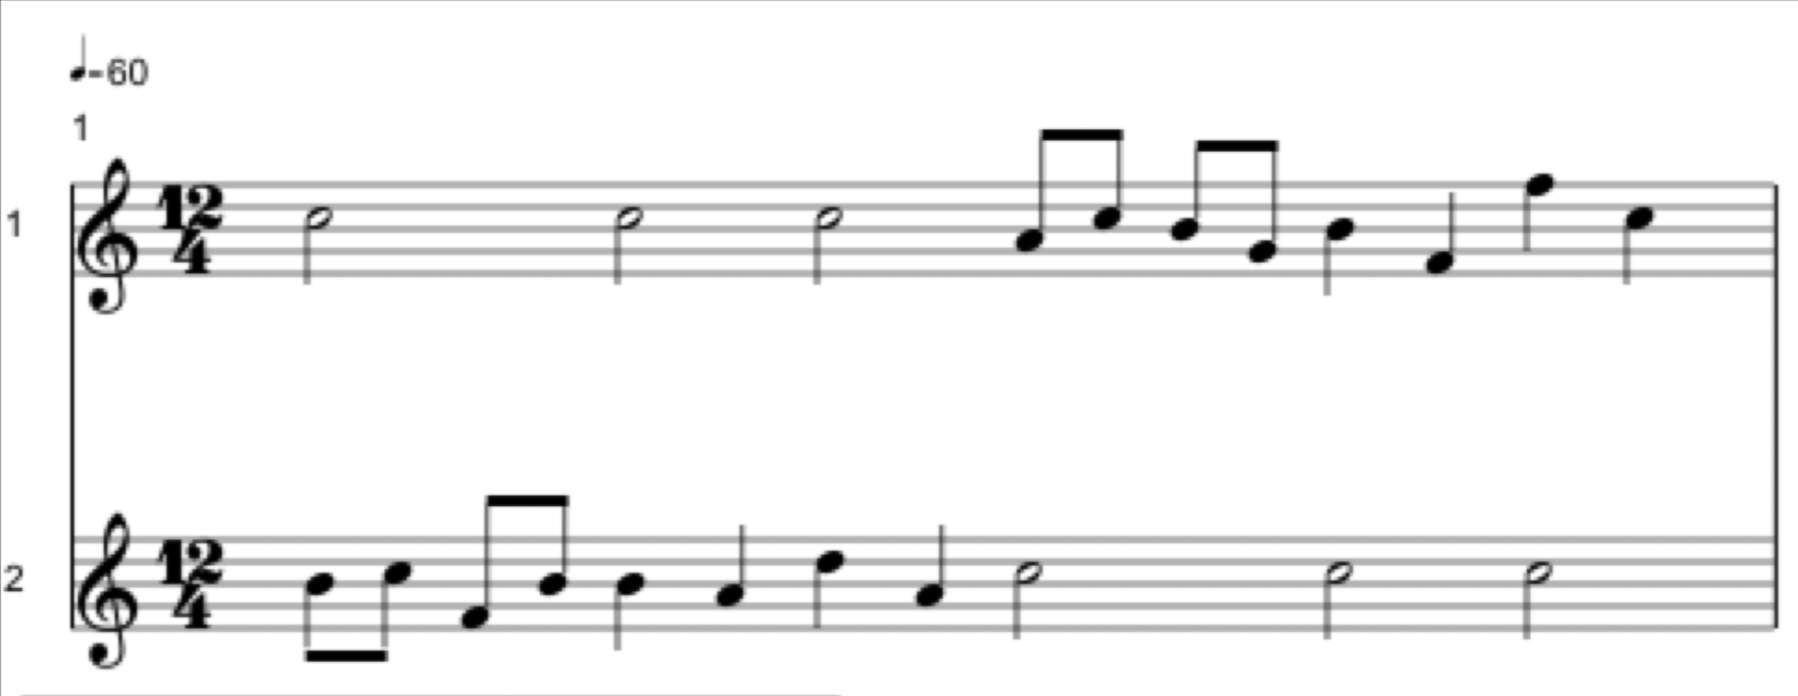
\includegraphics[width=0.9\textwidth]{maxscore-traditional.png} 
                \caption{A score with a random melody rendered in MaxScore’s default layout.
        \label{fig:maxscore-traditional}}
    \end{minipage}\hfill
    \begin{minipage}{0.45\textwidth}
        \centering
        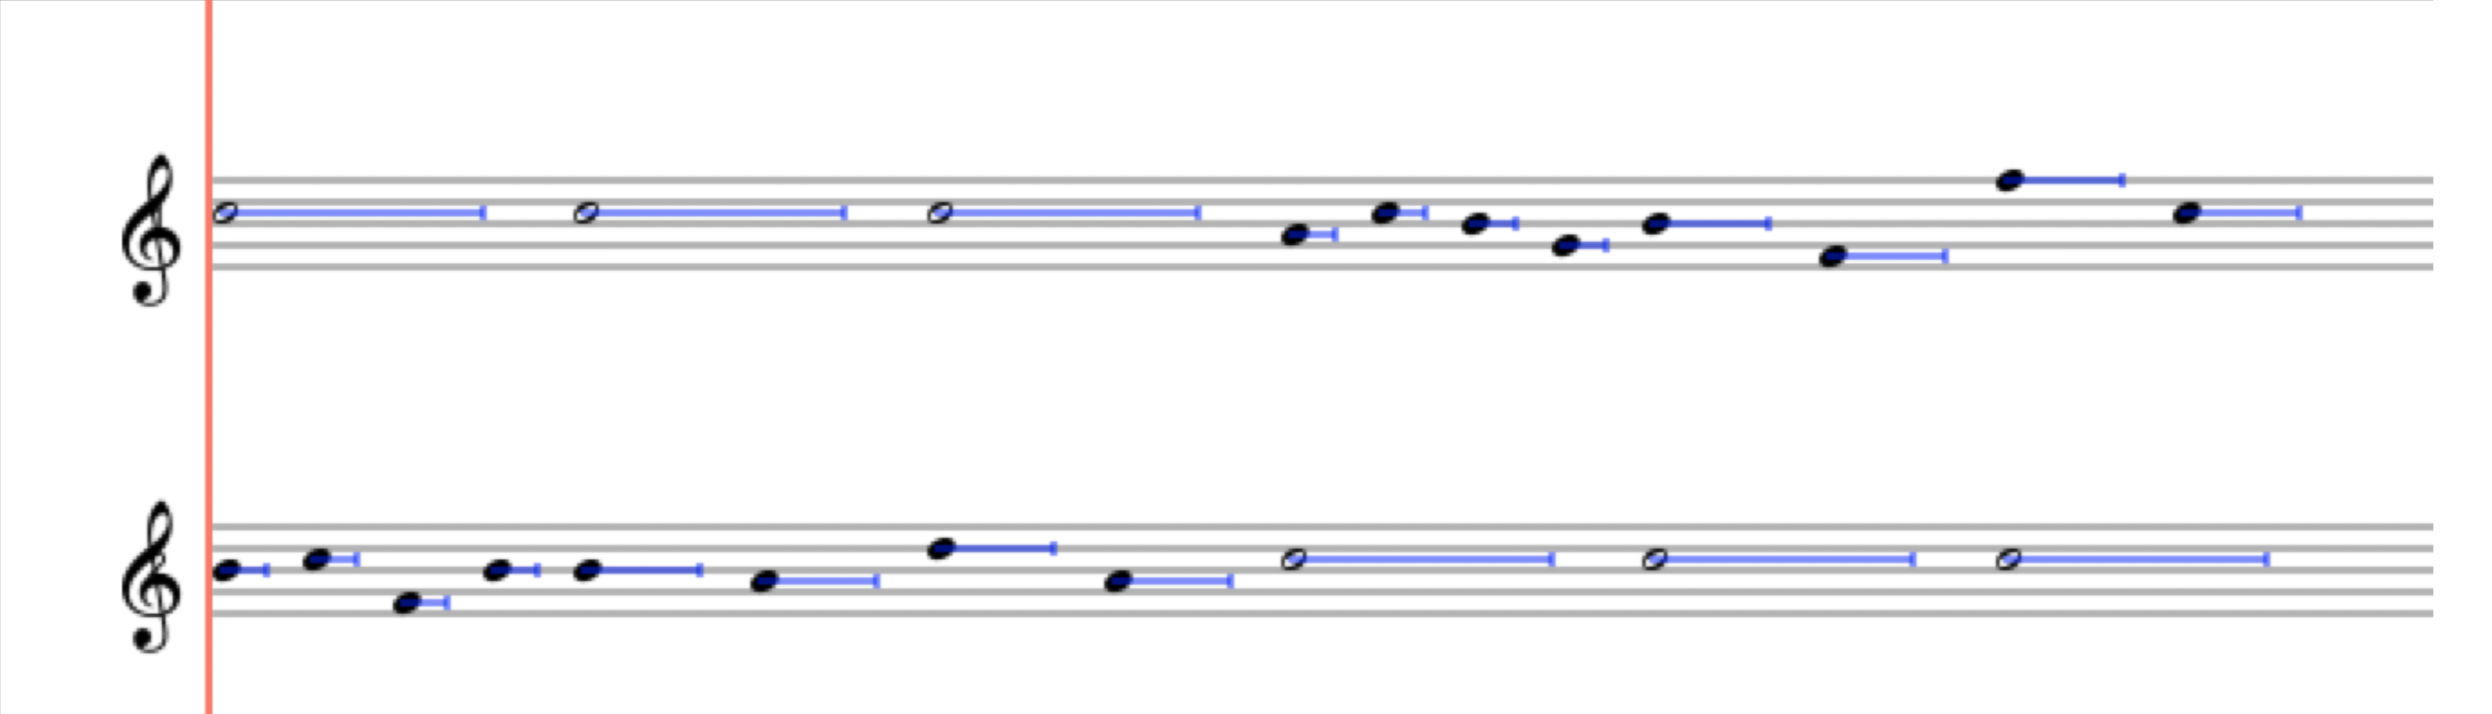
\includegraphics[width=1\textwidth]{maxscore-proportional.png} 
       	\caption{Same score after applying proportional notation. The default hold times indicated by the blue line is set to 80\% of the event’s nominal duration.
\label{fig:maxscore-proportional}}
    \end{minipage}
\end{figure*}

\section{Maxscore}
As mentioned in section~\ref{sec:foundations}., MaxScore possesses a fair amount of flexibility in terms of rendering to a wide array of targets. The JavaScript object render2Browser.js was created to facilitate the communication between the MaxScore object and the hfmt.drawsocket abstraction. The js object was designed with MNMP in mind. Such performances pose enormous difficulties when distributing large scores with dozens of staves. In performances with Quintet.net, scores containing just a few staves were split into instructions to be reassembled by individual instances of the MaxScore object and rendered locally by the Clients. But doing the same with dozen of instances (potentially destabilizing the environment and introducing unwanted latency), we resorted to a different strategy by implementing the concept of multi-client rendering, treating the ensemble of clients like one single canvas. In Maxscore, nearly every rendering message contains indexes referring to the notation object it represents  (Figure~\ref{fig:maxscore-mesages}). TThanks to those indexes, render2Browser.js is capable of dynamically reroute a rendering message to targets set by the staffgroups attribute. This attribute can have the following values: score, parts or a list containing either indexes (for individual staves), two indexes joined by hyphens (for a staff range) or any number of indexes joined by plusses (for arbitrary collections of staves) such as in this example: staffgroups 0 1-2 2 0+3.

In addition to splitting and routing messages, the object is also capable of respacing staves so that resulting layout looks acceptable. It does so by querying the MaxScore object during rendering to obtain crucial information about staff spacing and using this information to apply offsets to the y values of each message to be rendered.

\begin{figure}[h]
\centering
\begin{lstlisting}[ mathescape,
						columns=fullflexible,
						basicstyle=\oscfontsize\fontfamily{lmvtt}\selectfont,
						breaklines=true,
						 frame=single ]
tempoqtrequals 20. 21. 0.5 Measure 0. ...
tr 22. 75.959999 0.5 Staff 0. 0. staffnumber1 0. 63. 0.5 Staff 0. 0. timesig4 43. 57. 0.5 Staff 0. 0.
...
StaffLine 0. 0. 4. 0.5 20. 75. 300.660797 75. false
...
frgb 0 0 0
noteheadblack 83.620689 57. 0.5 Note 0. 0. 0. 0.
frgb 0 0 0
no_accidental 75.555557 57. 0.5 Note 0. 0. 0. 0.
frgb 0 0 0
stem 76.620689 79. 0.5 Note 0. 0. 0. 0. STEM_DOWN
RenderMessage staff 0 0 166. 13. 0.5 
rendered Picster-Element[5] 175.3ocUOsnBBCCCzOk6dAg[...]
\end{lstlisting}

\caption{A sample of rendering messages generated by the MaxScore object. 
\label{fig:maxscore-mesages}}
\end{figure}

Figure \ref{fig:maxscore-mesages} shows a sample of rendering messages generated by the MaxScore object. Note that nearly every message is accompanied by indexes (in red) referring to the notation object they represent. The y coordinates (blue numbers) are remapped according to the current staffgroups setting. The RenderMessage message contains a gzip’ed JSON object which in turn codes for a graphical score element such as a line, a rectangle, an arc or an image.

render2Browser.js is also capable of animating any number of cursors moving across set of measures and staves (see TENOR 2018 paper).

Figure x. A MaxScore score with 4 staves (top) rendered dynamically in four browser windows (center and bottom). The staves are split and grouped by render2Browser.js according to the following staffgroup settings: “0 1-2 2 0+3”.

To scroll the entire score horizontally, we created another JavaScript object called maxscore.proportionalNotation.js. It toggles between MaxScore’s default score layout and its proportional representation by hiding rests, stems, beams and naturals and indicating the duration of a note by a line extending from a note. The length of a measure is calculated by obtaining its tempo and time signature values and taking a setTimeUnit attribute into consideration. The durational scaling base value of 0.385 has proven to be optimal for spatially representing the delta time between events. The start message will cause a playhead to appear at the position given by the scoreLeftMargin attribute and instruct the browser to scroll the score. We are planning to also support scores created for the Decibel ScorePlayer in the future. 



%describe use of hfmt.drawsocket via Maxscore translation script.




\section{Case study}

A new  piece (Raindrops Keep Falling) by Georg Hajdu was premiered at the December 2018 WOCMAT conference in Hsinchu, Taiwan. This composition for clarinet, cello and percussion with multimedia consists of a transition between various rain samples and a late-1960’s hit called Raindrops Keep Fallin' on My Head mediated by a Max Pluggo effect called Raindrops. It’s also a tongue-in-cheek reference to the usual end-of-year weather pattern in Taiwan. The piece features 12 different versions of the song found on the Internet. The HfMT graduate student and research assistant James Cheung arranged the songs in such manner that they all share the same tempo structure and key signature, allowing the seamless navigation between those versions. James also created an arrangement of the song for the aforementioned instrumentation to be performed simultaneously with the recording, which was further subject to processing. First, parts of the score were “whited out” by a probabilistic process so that more and more events were allowed to appear paralleling a similar process applied to the audio tracks. The whiting-out was achieved by a JavaScript object called maxscore.whiteout.js capable of applying a “whiteout” gradient to a given section (the name was inspired by Cat Hope’s piece The Great White). Second, the score was turned into proportional notation, transmitted to the iPads of the performers via hfmt.drawsocket and scrolled in synch with the audio. The system held up to its promise as a computer-based conducting system. The scrolling was fluid and the musicians stayed in tempo despite the tempo fluctuations in the audio track. 
 
Figure x. Excerpt from Raindrops Keep Falling (2018) for clarinet, cello and drum set.



